\documentclass[../main.tex]{subfiles}
\begin{document}

\section{\label{sect:formalism}The Langevin method for real and complex variables}
%We need to do some research: read Aarts, Salcedo, Seiler and see what they say about the history
Stochastic quantization as a method for treating Euclidean field theories has been around since Parisi and Wu first proposed the connection between the Euclidean field theories and statistical systems coupled to a heat bath~\cite{ParisiWu}. It is now well-established as a successful tool for treating quantum many-body systems with a real Euclidean action~\cite{PhysicsReportsStochasticQuantization}. This section examines the method for systems without a sign problem (referred to from here on as ``real Langevin") and its extension to systems with complex actions as a possible circumvention of the sign problem (``complex Langevin" or CL, the focus of this review). We present a pedagogical example to illustrate the real and complex Langevin methods using a simple toy model, and discuss some of the challenges that arise in using the complex Langevin method along with proposed solutions to those problems.

%%%%%%%%%%%%%%%%%%%%%%%%%%%%%%%%%%%
\subsection{Complex Langevin: origins and modern re-emergence~\label{sect:CL}}
Shortly after the introduction of the concept of real stochastic quantization, it was realized that the approach could be extended to the case of complex actions.
Loosely speaking, using a Langevin equation rather than an importance sampling approach eliminates the restriction to real and positive semidefinite measures. This is due to the ability of the probability measure used in a Langevin method to be complexified -- at least formally. In 1983 such a strategy was discussed independently by Klauder~\cite{Klauder1983a,Klauder1983b} and Parisi~\cite{Parisi1983} as an alternative to existing Monte Carlo methods and marked the first investigations of how the complex Langevin equation can be used to address the complex phase problem.

The elegant form of the approach as well as the potential to circumvent the sign problem drew considerable interest in the years after the initial proposals. Following the first successful numerical application for the quantum Hall effect by Klauder \cite{Klauder1984}, the method was employed in many studies, albeit with mixed success. Unfortunately, the convergence of the method cannot be guaranteed a priori and even if convergence is achieved, spurious solutions with biased expectation values might be found. This is connected to subtle mathematical issues that arise in the case of complex weight and the structure of the associated complex Fokker-Planck equation. As a consequence, the initial flurry of interest stalled and progress on these matters slowed down over the years.
However, studies have investigated the applicability of CL to a set of toy problems~\cite{PRC2001026303} and interestingly the method has also spread to simulations of polymeric fluids \cite{Ganesan_2001,Fredrickson2002} and to reaction simulations in the context of physical chemistry \cite{HOCHBERG200654,DELOUBRIERE2002135} as a way to include beyond mean-field corrections.

As recently as the mid 2000s to early 2010s, the CL approach re-emerged as a method of interest in relativistic physics, particularly in QCD. In this new era, early applications to relativistic physics examined non-equilibrium QFT, which can provide insights into high-energy physics, particularly heavy ion collisions. Due to the non-perturbative nature of these non-equilibrium systems, standard approximation techniques fail. Lattice simulations provide a potential avenue for exploration, but these non-equilibrium systems do not lend themselves to a Euclidean treatment, and a Minkowski formulation suffers from a sign problem. In 2005, Berges and Stamatescu demonstrated the viability of CL to treat non-equilibrium QFT using first-principles simulations~\cite{PhysRevLett95202003}. Later work built on these results to examine how CL could lead to breakthroughs in our understanding of QCD plasmas in heavy-ion collisions, early thermalization, and other open questions in quantum field theory~\cite{PhysRevD75045007}.

In 2008, Aarts and Stamatescu demonstrated that CL could be applied to models of finite density QCD that exhibit a sign problem~\cite{JHEP200809018}. Shortly after that, Aarts demonstrated that CL could be used to circumvent the sign problem in the relativistic Bose gas with finite chemical potential~\cite{AartsPRL102131601, JHEP200905052}. This began a resurgence of interest in this method in the field of finite density Lattice QCD (LQCD), in which nonperturbative calculations of strongly interacting matter with finite baryon chemical potential are inhibited by the sign problem. This renewed interest led to work in the next few years on optimization of the method to prevent runaways and improve stability, using stochastic reweighting, gauge fixing, and adaptive step size algorithms~\cite{BERGES2008306,AARTS2010154,JHEP20100820}.

The successes of the method, and advances made in treating instabilities and singularities in the fermion determinant, have generated interest in applying CL to non-relativistic systems, particularly many-fermion systems, in which sign problems arise frequently. Work with the CL method in the context of non-relativistic systems is just beginning, but is already showing great promise. Discussion of these recent applications to relativistic and non-relativistic physical systems can be found in Secs.~\ref{sect:RQFT} and~\ref{sect:NRQFT}.

Despite the formal challenges of CL, it should be pointed out that, at least in principle, the existence of a well-defined probability measure on a complexified field space
is guaranteed under certain conditions (often referred to as Weingarten's theorem~\cite{PhysRevLett.89.240201}). However, the challenge lies in constructing such a measure, which has been investigated by Salcedo and others ~\cite{Salcedo:1996sa, Salcedo_2007, Wosiek:2015iwl, Wosiek:2015bqg, PhysRevD.94.074503, Seiler_2017, Salcedo_2018, Wosiek:2018jht}. While this is a very attractive area of research, we will not pursue it further in this review.


%%%%%%%%%%%%%%%%%%%%%%%%%%%%%%%%%%%
%%%%%%%%%%%%%%%%%%%%%%%%%%%%%%%%%%%
%%%%%%%%%%%%%%%%%%%%%%%%%%%%%%%%%%%
%%%%%%%%%%%%%%%%%%%%%%%%%%%%%%%%%%%
\subsection{Stochastic quantization: path integrals and the Langevin process}
%
The main ingredient of the CL method is the concept of {\it stochastic quantization}. The idea was introduced in the seminal 1981 paper of Parisi and Wu~\cite{ParisiWu} and a few years later summarized nicely in the famous review article by Damgaard and H\"{u}ffel~\cite{PhysicsReportsStochasticQuantization} \footnote{See also Ref.~\cite{jona-lasinio1985} for a more formal introduction to stochastic quantization}.
Notably, stochastic quantization has played an important role both theoretically as well as computationally; in particular, it has been used extensively in field theory (see e.g. Ref.~\cite{PhysRevD.32.2736}) and condensed matter
(see e.g. Ref.~\cite{PhysRevB.99.035114}), and is the precursor of the
hybrid Monte Carlo algorithm~\cite{Duane:1987de, PhysRevD.35.2531}, which has been the workhorse of LQCD for decades. In the following we present a brief introduction to
stochastic quantization in order to lay out the foundation for later considerations.

For a quantum field theory of a real field $\phi$ governed by a real action $S[\phi]$, stochastic quantization provides an intuitive way to understand path integrals of the form
\beq
  \label{Eq:PathIntegralSQ}
  \CZ = \int\CD\phi\ {\rm e}^{-S[\phi]}.
\eeq
 As a first step, we introduce a purely fictitious time variable $t$, which represents the direction of the stochastic evolution. This fictitious time evolution is then governed by a stochastic differential equation, namely the Langevin equation:
 \beq
   \label{Eq:Langevin_continuum}
   \frac{{\rm d}\phi}{{\rm d}t} = -\frac{\delta S[\phi]}{\delta \phi} + \tilde{\eta}.
 \eeq
The first term on the right hand side is called the drift term, also sometimes referred to as the classical flow as it constitutes the deterministic part of the time-propagation of the fields. The second term on the left hand encodes the random nature of the equation and is given by a white-noise with zero autocorrelation, i.e. $\tilde\eta \sim \delta(t-t')$.

For practical purposes it is convenient to rewrite this equation in a discrete form which can be done by integrating both sides over the time interval $\Delta t$. This leads to the discrete Langevin equation
%
\beq
  \label{Eq:Langevin}
  \Delta \phi = K[\phi] \Delta t + \eta,
\eeq
%
where $\eta$ is typically chosen to be a Gaussian random variable with $\langle \eta \rangle = 0$ and $\langle \eta^2 \rangle = 2\Delta t$. The angle brackets denote an
average over $\eta$. This random process will produce configurations $\phi$ that follow a certain probability distribution. The key ingredient of stochastic quantization
is the realization that the equilibrium distribution (if it exists) of the $d+1$ dimensional random process in \equref{Langevin} corresponds to the probability measure in the $d$-dimensional path integral \equref{PathIntegralSQ}. The extra dimension is simply the fictitious time $t$.

It is instructive to consider the above stochastic differential equation without the noise term. In that case, \equref{Langevin_continuum} reduces to an ordinary differential equation and its form is nothing but that of a gradient descent. Starting out at a random (non-pathological) state, this implies that the solution will converge to a stationary point of the action, which is the ``mean-field'' or classical solution. The simple interpretation of the noise term is that it represents quantum fluctuations around this classical solution. In order to reproduce the correct physics, we have to ``add the correct amount of fluctuations" which is set by the Fluctuation-Dissipation theorem. Thus, stochastic quantization can be viewed as a very explicit form of quantization.

%In order to obtain the desired expectation values we need to average the solutions of the random process, $\phi_\eta(t)$, over all different realizations of the noise
%%
%\beq
%  \ev{\CO[\phi_\eta(t)]} = \int{\rm d}\eta\ P[\eta,t] \CO[\phi_\eta(t)]
%\eeq
%%
%which we will refer to as the Langevin average. Alternatively, we may define a time-dependent probability measure $P[\phi,t]$ and write for the average
%\beq
%  \label{Eq:EVOprob}
%  \ev{\CO[\phi_\eta(t)]} = \int \mathcal D\phi\ P[\phi,t] \CO[\phi]
%\eeq
%where we exchanged the integral over the noise for an integral over configurations $\phi$. To establish the validity of such a Langevin average, we need to investigate the temporal behavior of the expectation value and show that the time-dependent probability distribution depends on $S[\phi]$ in the way dictated by \equref{PathIntegralSQ}, at least at large enough $t$. An instructive discussion can be found in \cite{PTPS1993CLSimulation}, which we will follow closely.

The random process results in a sequence of time-dependent configurations $\phi_\eta(t)$ distributed according to a
time-dependent probability measure $P[\phi,t]$. The expectation value of a given observable $\mathcal O[\phi]$ is then
given by
%
\beq
  \label{Eq:EVOprob}
  \ev{\CO[\phi_\eta(t)]} = \int \mathcal D\phi\ P[\phi,t] \CO[\phi].
\eeq
%
To establish the validity of such a Langevin average, we need to investigate the temporal behavior of the expectation value and show that the time-dependent probability distribution depends on $S[\phi]$ in the way dictated by \equref{PathIntegralSQ}, at least at large enough $t$. 
Such a property will justify the use of temporal averages along the Langevin evolution to estimate the true expectation values of the theory.
An instructive discussion can be found in \cite{PTPS1993CLSimulation}, which we will follow closely.




As a first step, we take the fictitious-time derivative of the expectation value
%
  \bea
  \label{Eq:PhiAvgSide}
  \frac{{\rm d} \ev{\CO[\phi_\eta(t)]}}{{\rm d}t} = \int \mathcal D\phi\ \frac{{\rm d} P[\phi,t]}{{\rm d}t} \CO[\phi].
\eea
%
Note, that only the probability distribution carries a fictitious-time dependence. Alternatively, we may perform the same fictitious-time derivative by expanding the observable to second order in its $\phi$ dependence
%
\beq
  \label{Eq:obs_expansion}
  {\rm d} \CO[\phi] = \frac{\delta \CO[\phi]}{\delta\phi} {\rm d} \phi + \frac{1}{2} \frac{\delta^2 \CO[\phi]}{\delta\phi^2} ({\rm d} \phi)^2.
\eeq
%
According to \equref{Langevin} we may write
%
\beq
  \label{Eq:LEdiff}
  {\rm d}\phi = -\frac{\delta S[\phi]}{\delta\phi} {\rm d}t + {\rm d}w\, ,
\eeq
%
where ${\rm d}w$ is the so-called {\it Wiener increment} with the property
%
\beq
  \langle {\rm d}w^2 \rangle = \int_{t}^{t+dt} {\rm d}\tau\ \int_{t}^{t+dt} {\rm d}\tau'\ \langle \eta(\tau)\eta(\tau') \rangle = 2 \, {\rm d}t \, ,
\eeq
%
and vanishing mean $\langle{\rm d}w\rangle = 0$.
Substituting in \equref{obs_expansion} and using the properties of ${\rm d}w$ yields
\bea
  \langle {\rm d} \CO[\phi] \rangle = \left\langle  -\frac{\delta \CO[\phi]}{\delta\phi}\frac{\delta S[\phi]}{\delta\phi} + \frac{\delta^2 \CO[\phi]}{\delta\phi^2}  \right\rangle{\rm d}t\, ,
\eea
%
which allows us to write
%
\beq
  \frac{{\rm d} \langle \CO [\phi_\eta(t)] \rangle}{{\rm d} t} =
  \left\langle  -\frac{\delta \CO[\phi]}{\delta\phi}\frac{\delta S[\phi]}{\delta\phi} + \frac{\delta^2 \CO[\phi]}{\delta\phi^2}  \right\rangle
  \equiv \ev{L O}\, ,
\eeq
%
where we defined the so-called Langevin operator
%
\beq
  L_{r} = \int{\rm d}\tau{\rm d}^dx\ \left(\frac{\delta}{\delta\phi} + K[\phi]\right)\frac{\delta}{\delta\phi}\, ,
\eeq
%
with the drift $K[\phi] = -\frac{\delta S[\phi]}{\delta\phi}$, according to \equref{Langevin}. We may again write this as an integral over configurations
%
\begin{align}
  \frac{{\rm d}  \langle \CO [\phi_\eta(t)] \rangle}{{\rm d} t} &= \int \mathcal D \phi \left( -\frac{\delta \CO[\phi]}{\delta\phi}\frac{\delta S[\phi]}{\delta\phi} + \frac{\delta^2 \CO[\phi]}{\delta\phi^2}\right)P[\phi,t] \\
  &= \int \mathcal D\phi \ \CO[\phi] \left(\frac{\delta}{\delta \phi}\frac{\delta S[\phi]}{\delta \phi}  + \frac{\delta^{2}}{\delta \phi ^{2}}\right) P[\phi,t].
\end{align}
%
where the second line results from partial integration. Here we made the important assumption that the probability vanishes at the boundaries (or decays fast enough if the integration region is non-compact). These assumptions are in fact crucial and will be discussed in more detail below.

Comparing the above equation with \equref{PhiAvgSide} yields the Fokker-Planck (FP) equation:
%
\bea
  \label{Eq:FPE}
  \frac{\rm d}{{\rm d}t}P[\phi,t] = L_{r}^{\rm T} P[\phi,t]\, ,
\eea
%
with the formal adjoint of the above Langevin operator
%
\beq
L_{r}^{\rm T} \equiv \int{\rm d}\tau{\rm d}^dx\ \frac{\delta}{\delta \phi}\left(\frac{\delta}{\delta \phi} - K[\phi]\right) ,
\eeq
%
which is also referred to as the FP operator or FP Hamiltonian. To show that the stationary solution of this equation is indeed our desired probability distribution we perform similarity transformation
%
\beq
\label{Eq:PtildeP}
  \widetilde{P}[\phi,t] = {\rm e}^{S[\phi]/2} P[\phi,t] \, ,
\eeq
%
to rewrite the FP equation
%
\beq
  \frac{{\rm d}}{{\rm d}t}\widetilde{P}[\phi,t] =  \widetilde{L}_{r}^{\rm T}\widetilde{P}[\phi,t] \, ,
\eeq
%
with
%
\beq
  \widetilde{L}_{r}^{\rm T} = {\rm e}^{S[\phi]/2}\,L_{r}^{\rm T}\,{\rm e}^{-S[\phi]/2} =
  \int{\rm d}\tau{\rm d}^dx\ \left(- \frac{\delta}{\delta \phi} + \frac{1}{2}K[\phi]\right)
    \left(\frac{\delta}{\delta \phi} + \frac{1}{2}K[\phi]\right).
\eeq
%
This last equation reveals that, with a real action $S[\phi]$, our modified FP Hamiltonian is a self-adjoint and positive semidefinite operator, with a unique FP ground state $\psi_0 = {\rm e}^{-S[\phi]/2}$ and vanishing FP energy $E_0 = 0$.
We can therefore project our probability over the complete set of eigenfunctions and non-negative eigenvalues of
$\widetilde{L}_{r}^{\rm T}$, and see that our probability collapses to the ground state in the long time limit:
%
\bea
  \label{Eq:ProbFPE}
  \widetilde{P}[\phi,t] = \sum_{n = 0}^{\infty}a_{n} \psi_{n} {\rm e}^{-E_{n} t}\  \xrightarrow{t\to\infty}\ a_{0} {\rm e}^{-S[\phi]/2}.
\eea
%
Upon performing the back-transformation according to \equref{PtildeP} we obtain
%
\beq
  \lim_{t\to\infty} P[\phi,t] \sim {\rm e}^{-S[\phi]} \, ,
\eeq
%
which shows that the Langevin equation produces field configurations distributed according to the Boltzmann weight ${\rm e}^{-S[\phi]}$ in the limit of large fictitious time \footnote{We have assumed here that the spectrum of $\widetilde{L}_{r}^{\rm T}$ is discrete, which may not be true in practice. This assumption can be relaxed but it is important that the $E_0 = 0$ eigenvalue be non-degenerate.}.

%In practice it may be costly to obtain a sufficient number of solutions $\phi_\eta(t)$ at appropriately large $t$. 
The above justifies the use of temporal averages to estimate equilibrium expectation values. 
In fact, expectation values are obtained in practice by integrating over a time $T$:
%
\bea
  \langle \mathcal{O}\rangle \approx \frac{1}{T} \int_{t_{\rm th}}^{t_{\rm th}+T} {\rm d}t\ \mathcal{O}[\phi_\eta(t)],
\eea
%
where $t_{\rm th}$ reflects the equilibration time that is needed to approach the stationary probability distribution.



%%%%%%%%%%%%%%%%%%%%%%%%%%%%%%%%%%%
%%%%%%%%%%%%%%%%%%%%%%%%%%%%%%%%%%%
%%%%%%%%%%%%%%%%%%%%%%%%%%%%%%%%%%%
%%%%%%%%%%%%%%%%%%%%%%%%%%%%%%%%%%%
%%%%%%%%%%%%%%%%%%%%%%%%%%%%%%%%%%%
\subsection{A practical guide to real Langevin}
The above procedure is a well-established method for real-valued fields $\phi$ on a real manifold $\mathcal{M}$. In the following, we connect the concept with conventional Monte Carlo approaches based on Markov chains and highlight the similarities of these approaches in a practical way.

Generally, we are interested in expectation values of a given (Euclidean) field theory of the form of \equref{EVOprob}:
%
\beq
  \langle \CO \rangle = \frac{1}{\mathcal Z}\int{\mathcal D \phi\ \CO[\phi] {\rm e}^{-S[\phi]}} \equiv \int{\mathcal D \phi\ \CO[\phi] P[\phi]}.
  \label{Eq:langevin_toy_expectation}
\eeq
%
Typically, the evaluation of such high-dimensional path integrals is achieved by stochastic sampling, i.e. by producing a sequence of random states $\phi$ (interchangeably called samples or configurations). However, rather than producing a random state from scratch at every step (which might be expensive), new states are obtained by changing or {\it updating} an existing one. This can be written in the generic form
\beq
  \label{Eq:markov_chain}
  \phi_{n+1} = F[\phi_n]\, ,
\eeq
where the sample $\phi$ may be any representation of a physical state\footnote{In fact, finding suitable and efficient updates is a crucial part in devising any useful Monte Carlo method.}. If the next state is only dependent on the current one and not on any previous states the process is called ``memoryless" and the sequence of random samples represents a so-called ``Markov chain". This is the basis of the vast majority of most conventional Monte Carlo methods (often dubbed Markov-Chain Monte Carlo (MCMC) methods).

The Langevin method can be understood as such an approach, as we can see by recasting \equref{Langevin} into the form of \equref{markov_chain}:
\beq
  \label{Eq:discrete_langevin}
  \phi_{n+1} = \phi_{n} - \frac{\delta S[\phi]}{\delta\phi}\bigg|_{\phi=\phi_n}\Delta t + \sqrt{2\Delta t}\, \eta \, .
\eeq
%
By virtue of the discussion in the previous section, we know that in the long-time limit the samples $\{\phi_n\}$ follow the desired probability distribution $P[\phi]$ from \equref{langevin_toy_expectation}. Therefore, the strategy to evaluate the random sequence is identical to the one in regular Monte Carlo approaches: after starting out from a randomly produced configuration, we let the sampling process equilibrate for a certain thermalization time (typically a few multiples of the autocorrelation time -- see below) before we start to collect samples. An unbiased estimator of the expectation value with a total number of samples $N$ is then given by
%
\beq
  \label{Eq:mc_average}
  \langle \CO \rangle \approx \frac{1}{N} \sum_{i=1}^{N}{\CO[\phi_i]}\, ,
\eeq
%
and the statistical uncertainty (i.e., the variance of the mean) is estimated by
%
\beq
  \label{Eq:mc_error}
  \sigma_L = \sigma \sqrt{\frac{1 + 2\tau_a}{N}}.
\eeq
%
Here, $\sigma$ denotes the standard deviation of the set of values $\{ \CO[\phi_i]\}$ and $\tau_a$ is the integrated autocorrelation time, which reflects the (statistical) dependence of samples over the their Langevin-time history\footnote{For any Markov chain method, estimation of $\tau_a$ might be a challenging task depending on the number of accessible samples. Techniques such as bootstrap and jackknife can be used to obtain a reliable error estimate that considers the statistical dependence of the samples. An educational summary can be found in Ref.~\cite{Troyer2012}.}. From this expression we can also deduce that the number of samples is proportional to the elapsed Langevin time and the same conclusion holds: a longer Langevin evolution will result in better statistics and hence a smaller error bar.

It is important to note that the statistical uncertainty is not the only source of error, as we have introduced a systematic bias through the discretization of the Langevin equation in \equref{Langevin}. Results must then be extrapolated to the limit of $\Delta t\to 0$~\footnote{Notably, the hybrid Monte Carlo algorithm, mentioned above as a close cousin of RL, avoids this extrapolation in fictitious time by using Metropolis accept/reject steps. This property, however, does not imply that hybrid Monte Carlo can operate at arbitrarily large step sizes.}. The discretization of the Langevin equation presented above, which corresponds to Euler integration, leads to a linear dependence on the integration step $\Delta t$. Higher-order integrators can be designed if the noise term is appropriately accounted for, as investigated within RL in Refs.~\cite{DRUMMOND1983119, HOROWITZ1987510, CATTERALL1991177} and later extended to the complex case in Ref.~\cite{Aarts2012SU3}. Within the studied model, these extensions showed great success in reducing computational cost at equal systematic bias as well as to bring finite-step dependence below the statistical uncertainty. It is noted, however, that the majority of stochastic quantization studies still rely on the linear discretization as it is often sufficient to obtain useful results at modest computational effort.
%
\begin{figure}[t!]
  \centering
  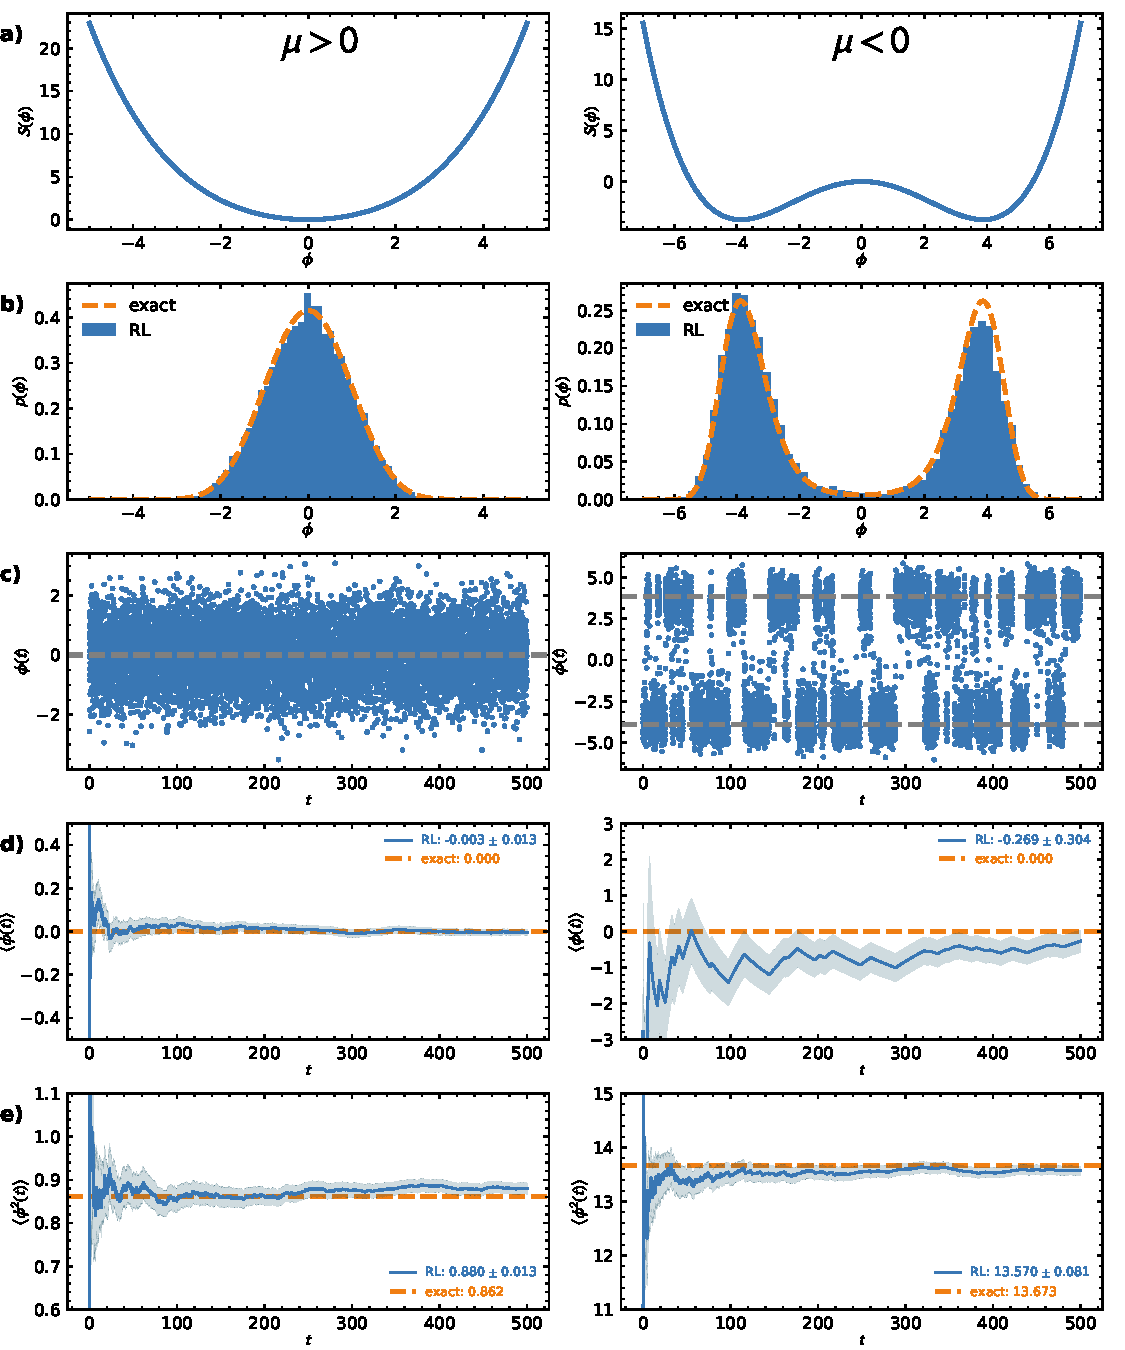
\includegraphics[width=\columnwidth]{./3mathunderpinnings/sq_toy_problem.pdf}
  \caption{\label{fig:sq_toy}(a) Action as a function of the real variable $\phi$. (b) Probability distribution ${\rm e}^{-S[\phi]}$ (dashed lines) along with the sampled histogram (bins). (c) Measured values of $\phi$ as a function of Langevin time. (d) Running average of $\langle \phi \rangle$ compared to the exact solution (orange dashed line) (e) Running average of $\langle \phi^2 \rangle$ compared to the exact solution (orange dashed line).}
\end{figure}
%

%%%%%%%%%%%%%%%%%%%%%%%%%%%%%%%%%%%
%%%%%%%%%%%%%%%%%%%%%%%%%%%%%%%%%%%
%%%%%%%%%%%%%%%%%%%%%%%%%%%%%%%%%%%
%%%%%%%%%%%%%%%%%%%%%%%%%%%%%%%%%%%
%%%%%%%%%%%%%%%%%%%%%%%%%%%%%%%%%%%
\subsubsection{Toy problem I: a pedagogical example of real Langevin \label{sect:sq_toy_real}}
%
In order to illustrate the RL method in a concrete numerical setting, we consider a simple integral as a toy problem for a $0 + 0$-dimensional field theory (i.e., the field $\phi$ depends neither on space nor time). Note that here we are not interested in a detailed study of the specific model at hand but rather aim to investigate the behavior of the RL method in a straightforward case. Of course it is highly inefficient to use RL for the solution of this simple problem, however, the section serves as a basic example of an application of the method. Furthermore, conclusions that generalize to more involved problems can be drawn by these simple considerations.

In this case, we consider the action
%
\beq
  S(\phi)\ =\ \frac{\mu}{2}\phi^2\ + \ \frac{\lambda}{4!}\phi^4,
  \label{Eq:langevin_toy_continuum}
\eeq
%
with real couplings $\mu$ and $\lambda$. In the spirit of a real field theory, we will keep $\lambda$ positive and thus end up with two distinct scenarios: one in which $\mu >0$ (the single well anharmonic potential) and one in which $\mu <0$ (the double well potential).

We readily derive the discrete Langevin equation for our toy-problem, according to \equref{discrete_langevin}:
%
\beq
  \phi_{n+1} = \phi_{n} - \left(\mu\phi_{n} + \frac{\lambda}{6}\phi_{n}^3\right)\Delta t\ +\ \sqrt{2\Delta t} \;\eta,
  \label{Eq:langevin_toy_discrete}
\eeq
%
where $\eta$ denotes a standard Gaussian white noise. In principle, this is everything needed to calculate expectation values of the form \equref{mc_average}.


In \figref{sq_toy}, a detailed analysis of two simulations at fixed $\lambda = 0.4$ and $\mu = \pm 1$ is presented (left and right columns, respectively). The second row from the top shows the histograms of the sampled field values, which should follow the distribution ${\rm e}^{-S[\phi]}$ (exact solution shown with dashed lines) in the limit of large Langevin time $t \rightarrow \infty$. While in the single-well system (left column) this is the case to a good approximation, it is apparent that the double-well scenario still suffers from a slight asymmetry. This can occur when the random process gets ``stuck" in an area of configuration space and does not easily move to another high probability area of configuration space (i.e. the other well).

This behavior can be further elucidated by the measured field values as a function of $t$ [row (c)]: on the left we see white noise centered around the expected value of $0$ while on the right we observe several correlated plateaus, corresponding to either the negative or the positive well. Ultimately, this behavior leads to a signal-to-noise issue in the calculation of the expectation value $\langle \phi \rangle$, reflected by large statistical uncertainties for the double well case [right column of row (d)].  Due to the symmetry of the problem, however, the running average for $\langle \phi^2 \rangle$ converges to the exact value relatively smoothly in both cases. Thus, by investigating one observable no profound statements can be made about a different one. While the autocorrelation of observable $A$ may be small and its statistical errors under control, observable $B$ could display erratic behavior and suffer from extremely slow convergence.

By tuning the parameters of the model, one could even study the extreme case where the two wells are separated by a barrier that cannot be surmounted by the random walk
(signaling a breakdown of ergodicity, a topic that we will return to below). In such a situation, the expectation value $\langle \phi \rangle$ would indicate that the discrete symmetry is broken, which certainly is not a physical result for our model. This reflects the problem of meta-stability of any Markov chain method, which is often very hard to detect {\it a priori}. Generally, one needs to address this issue carefully in real simulations, for example by sweeping numerical parameters in a systematic manner.

% Autocorrelation & step size dependence part.
\begin{figure}[t]
  \centering
  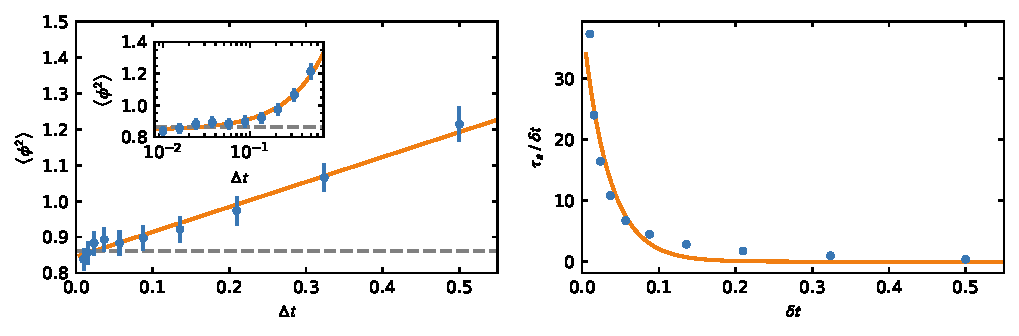
\includegraphics[width=\columnwidth]{./3mathunderpinnings/real_plot.pdf}
  \caption{\label{fig:sq_stepsize} Real Langevin results for the simulation parameters $\mu=1$, $\lambda=0.4$ and a total Langevin-time of $10^3$. (Left) Symbols reflect RL results for  $\langle\phi^2\rangle$ along with the statistical errorbars as a function of integration time step $\Delta t$. The dashed line represents a linear extrapolation to the limit $\Delta t\rightarrow 0$ (horizontal dashed line). (Inset) Same data on a semi-log scale. (Right) Integrated autocorrelation time of $\phi^2$ in units of the time step as a function of $\Delta t$.}
\end{figure}
%
Finally, by inspecting the Langevin equation in \equref{langevin_toy_discrete} it becomes apparent that the autocorrelation time between samples $\tau_a$ should be inversely proportional to the Langevin time step $\Delta t$, i.e., statistically independent samples will be more expensive as the integration step decreases. On the other hand, a coarser integration step will yield a larger systematic error and thus a balance must be found where both the computational effort as well as the precision are within reasonable bounds.
This behavior is illustrated in \figref{sq_stepsize}, where we show the dependence for $\langle\phi^2\rangle$ as well as $\tau_a$ on the integration stepsize $\Delta t$. Indeed, we observe a systematic linear behavior of $\langle\phi^2\rangle$, which is expected due to the order of the Langevin equation (see discussion in the previous section). Further, also the integrated autocorrelation $\tau_a$ shows the expected behavior: it increases as the integration step approaches $0$.



%%%%%%%%%%%%%%%%%%%%%%%%%%%%%%%%%%%
%%%%%%%%%%%%%%%%%%%%%%%%%%%%%%%%%%%
%%%%%%%%%%%%%%%%%%%%%%%%%%%%%%%%%%%
%%%%%%%%%%%%%%%%%%%%%%%%%%%%%%%%%%%
%%%%%%%%%%%%%%%%%%%%%%%%%%%%%%%%%%%
\subsection{A practical guide to complex Langevin}

Thus far we have seen that the concept of stochastic quantization works well, given that the action $S[\phi]$ is real, i.e. when there is no sign problem. But what about the much more general and interesting case of complex-valued actions? In that case, the probability distribution in \equref{EVOprob} becomes a {\it complex} distribution
%
\beq
  \label{Eq:complex_p}
\rho[\phi] = \frac{{\rm e}^{-S[\phi]}}{\mathcal Z},
\eeq
%
while the field $\phi$ is still a real quantity. With such an action, a single step in the Langevin process according to \equref{discrete_langevin} would result in an imaginary component for $\phi$. At least from a practical perspective, as remarked by Parisi, ``nothing forbids to write a Langevin equation also for complex actions'' \cite{ParisiWu}.
Formal aspects aside (we return to those below), the idea is that one may perform calculations by extending the real stochastic process described above to a complex one. For a theory governed by a complex action $S[\phi]$, CL extends the target manifold of the field $\phi(x)$ to the complex plane by setting
%
\beq
  \phi \to \phi_{R} + i \phi_{I},
\eeq
%
and analytically extending the domain of the action functional:
%
\beq
S[\phi] \to S[\phi_{R} + i \phi_{I}].
\eeq
%
Naturally, a necessary condition for this extension to be valid is that $S[\phi]$ must be a holomorphic function of $\phi$.

The two Langevin methods -- real and complexified -- are compared side-by-side in \figref{SQCL}.
With such an extension, the CL method proceeds very much in the same way as the real Langevin method, but now with a double system of coupled stochastic differential equations:
%
\bea
  \Delta \phi_{R} &=& K_{R}\Delta t + \eta_{R}(t),\\
  \Delta \phi_{I} &=& K_{I}\Delta t + \eta_{I}(t) ,
\eea
%
where the real and imaginary drift functions $K_{R}$ and $K_{I}$ are found by taking the real and imaginary parts of the functional derivative of the complex action:
%
\bea
  K_{R} &= -\textnormal{Re}\left[\frac{\delta S[\phi]}{\delta \phi}\right],\\
  K_{I} &= -\textnormal{Im}\left[\frac{\delta S[\phi]}{\delta \phi}\right].
\eea
%
The real and imaginary noise obey the properties shown in \figref{SQCL}.
%
%\bea
%\langle \eta^2_{R} \rangle = 2 N_{R} \Delta t \\
%\langle \eta^2_{I} \rangle = 2 N_{I} \Delta t\\
%N_{R} - N_{I}  = 1\\
%\langle \eta_{R} \rangle = \langle \eta_{I} \rangle = 0.
%\eea
%
It is important to note that, while the amplitudes of the real and imaginary noise terms are related, the two Wiener processes are completely independent. In practice, the imaginary noise is usually set to zero, which satisfies the constraints shown in \figref{SQCL} and it has been found to have the best numerical properties~\cite{AartsPRD81054508}. Finally, it should be pointed out that,
beyond the complexification of each real degree of freedom, the above (coupled) Langevin processes are themselves real. We return to the justification for CL and related challenges after giving an illustrative example.
%
%
\begin{figure}[t]
  \centering
  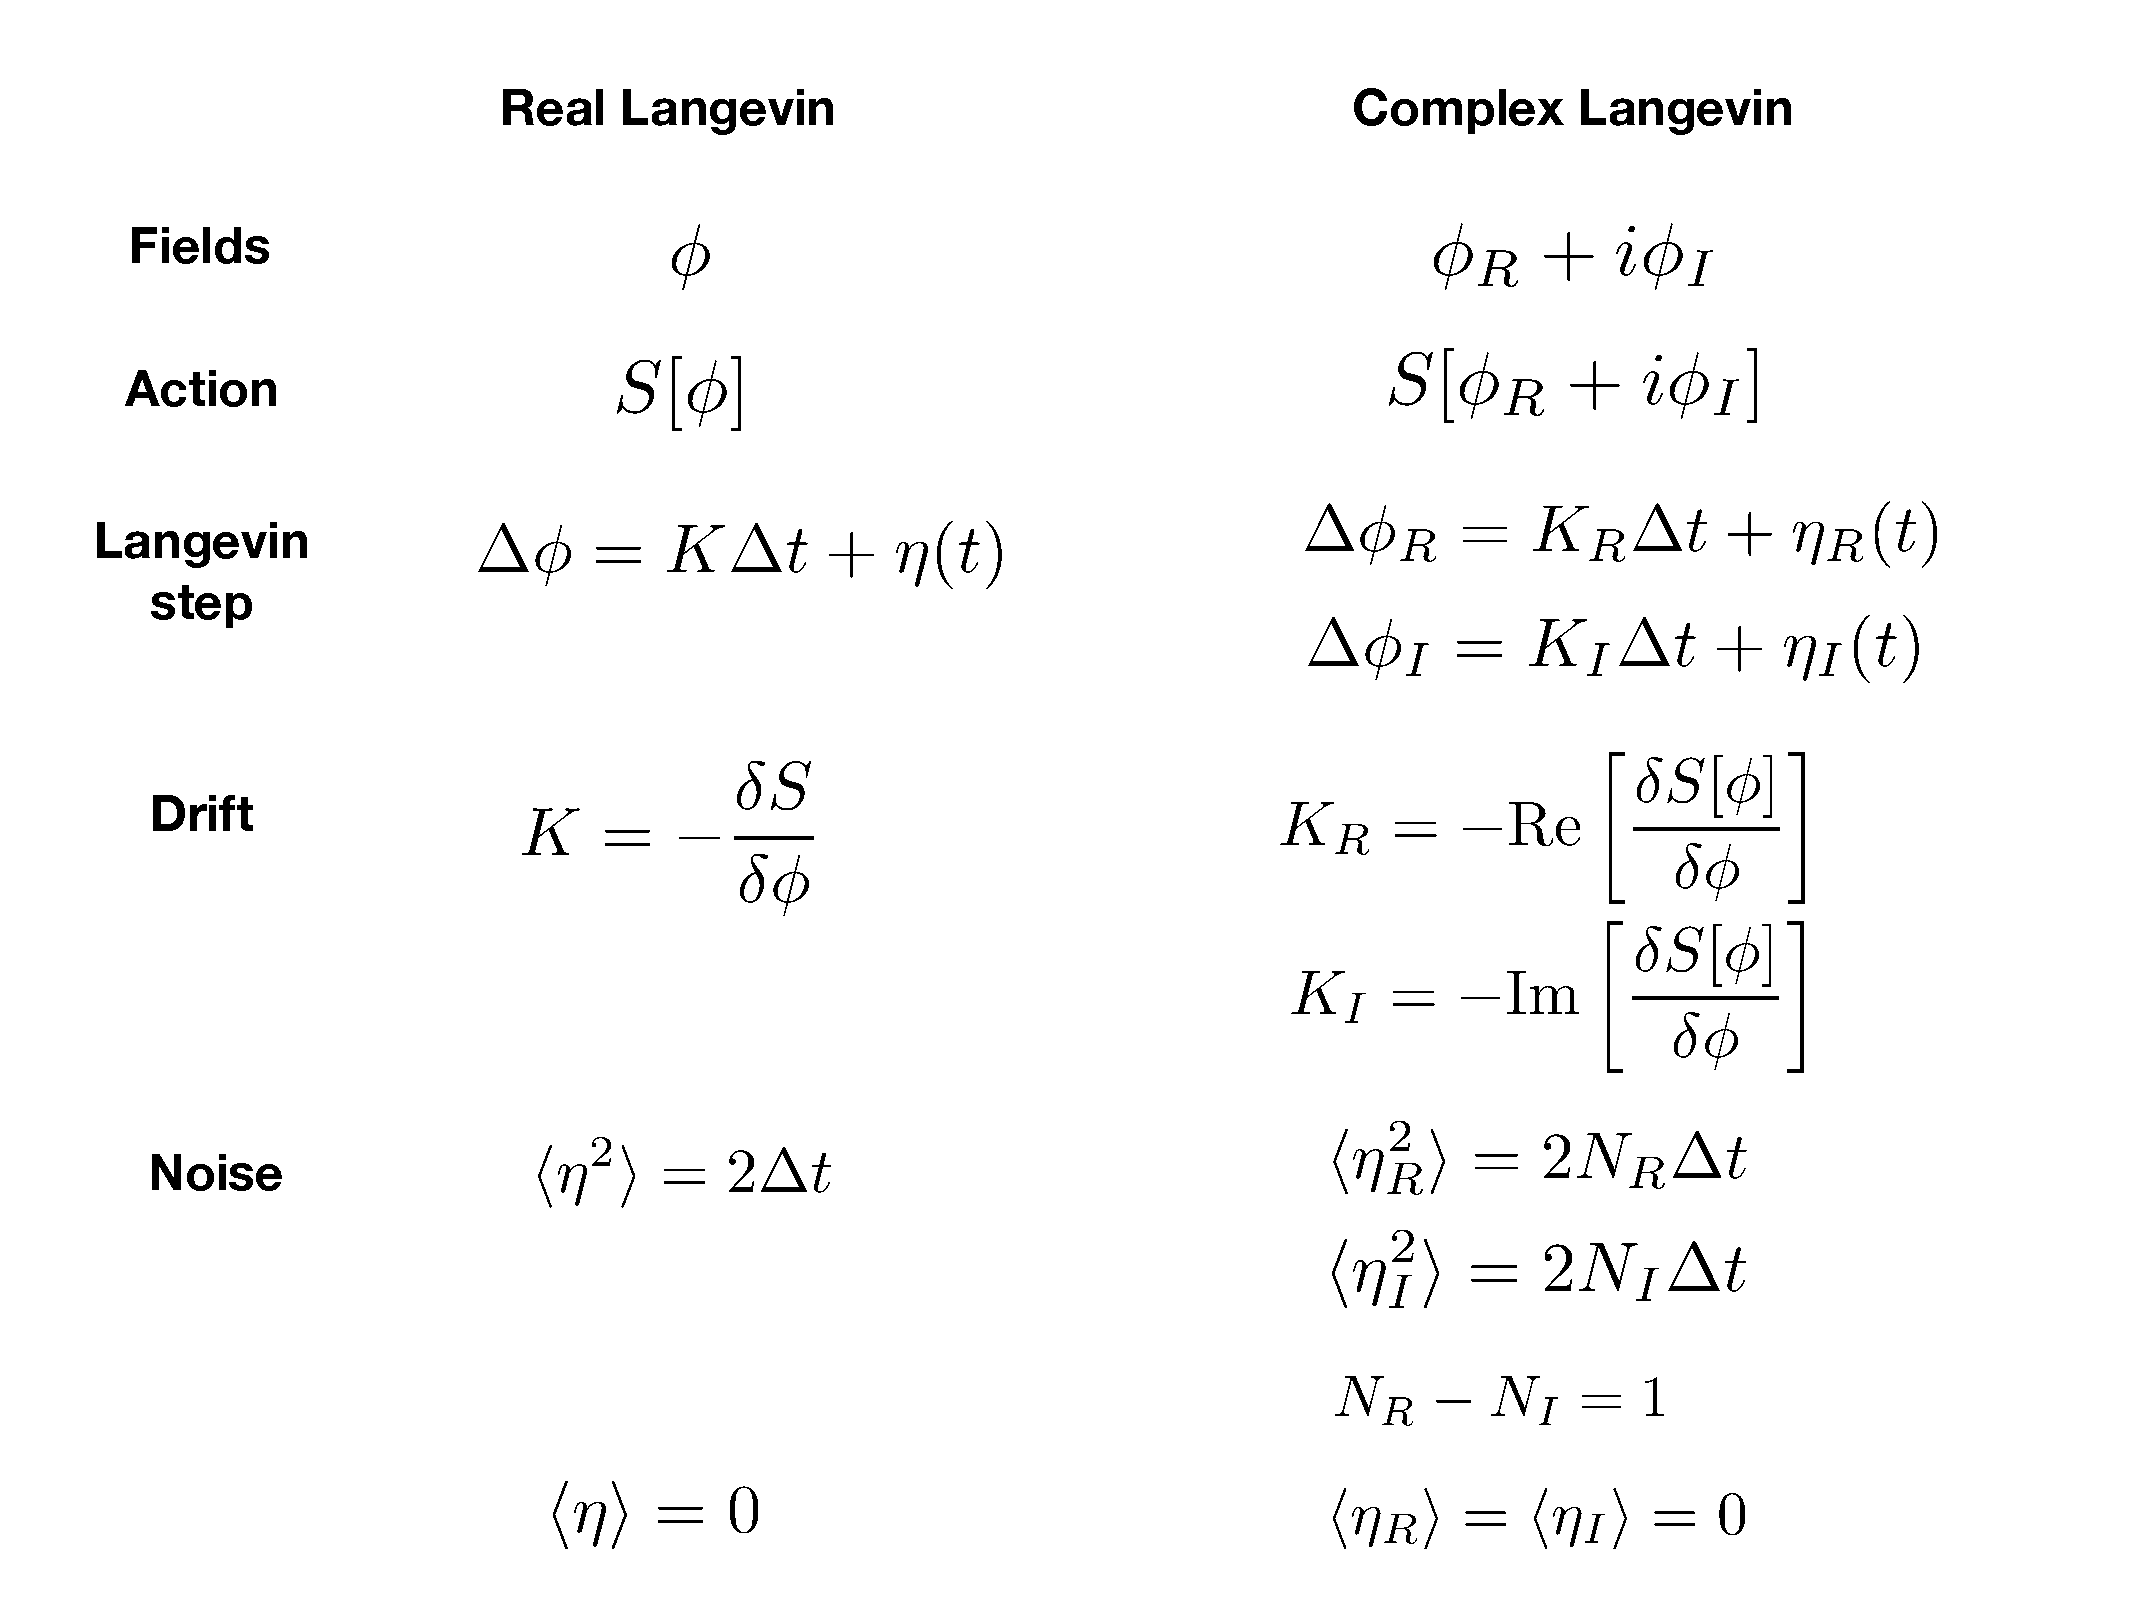
\includegraphics[width=0.7\columnwidth]{./3mathunderpinnings/RLvsCLTable.pdf}
  \caption{\label{fig:SQCL} The Langevin method with real-valued fields versus complex-valued fields}
\end{figure}
%

%%%%%%%%%%%%%%%%%%%%%%%%%%%%%%%%%%%
%%%%%%%%%%%%%%%%%%%%%%%%%%%%%%%%%%%
%%%%%%%%%%%%%%%%%%%%%%%%%%%%%%%%%%%
%%%%%%%%%%%%%%%%%%%%%%%%%%%%%%%%%%%
%%%%%%%%%%%%%%%%%%%%%%%%%%%%%%%%%%%
\subsubsection{Toy problem II: a pedagogical example of complex Langevin\label{sect:sq_toy_complex}}
  In order to see the CL machinery at work we build on the toy-problem in \secref{sq_toy_real}. Indeed, from a computational standpoint, CL is largely just the Langevin process of stochastic quantization with complex variables.

  The most natural route towards a complex field theory would of course be to consider complex valued couplings $\mu$ and $\lambda$ in \equref{langevin_toy_continuum}, which in fact has been considered before, see e.g. \cite{PTPS1993CLSimulation}. However, this would amount to solving a different theory as the couplings necessarily take on different values. Alternatively, we may rewrite the above problem with a suitable Hubbard-Stratonovich transformation which merely amounts to an alternative representation of the same physical scenario. Moreover, this is very much in the spirit of real-world problems, where a HS-transform is often used to integrate out fermionic degrees of freedom.
  To achieve this, we insert a suitable factor of $1$ into the partition function in terms of an auxiliary variable $\sigma$:
  \bea
    \CZ &=& \int_{-\infty}^{\infty} {\rm d}\phi\ {\rm e}^{-S(\phi)} \\
        &=& \sqrt{\frac{\lambda}{24\pi}}\ \int_{-\infty}^{\infty} {\rm d}\sigma\ \exp\left( -\frac{\lambda}{24} \sigma^2 \right)\
          \int_{-\infty}^{\infty} {\rm d}\phi\ \exp\left[ - \left( \frac{\mu}{2}\phi^2 + \frac{\lambda}{24}\phi^4\right) \right].
  \eea
  A shift $\sigma\rightarrow\sigma + i\phi^2$ allows us to write
  \beq
      \mathcal{Z} = \sqrt{\frac{\lambda}{24\pi}} \int_{-\infty}^{\infty} \d\sigma \int_{-\infty}^{\infty}\d\phi\
          \exp\left[ -\left( \phi^2 \left( \frac{\mu}{2} + \frac{i\lambda\sigma}{12} \right) + \frac{\lambda}{24}\sigma^2 \right) \right]\, ,
  \eeq
  and subsequently to integrate out the dependence on the old field $\phi$ (note that this is only possible in the case $\textnormal{Re}[\mu] > 0$). Ultimately we obtain the ``bosonized" version
  \beq
    \label{Eq:cl_bosonized_z}
    \mathcal{Z} = \int_{-\infty}^{\infty} \d\sigma \exp\left[ - \left( \frac{\lambda}{24}\sigma^2 - \frac{1}{2}\log\frac{\lambda}{12\mu + 2i\lambda\sigma} \right) \right] \equiv \int_{-\infty}^{\infty} \mathrm{d}\sigma\, {\rm e}^{- S_\mathrm{B}(\sigma)}\, ,
  \eeq
  where we defined the ``bozonized action"
  \beq
    S_\mathrm{B}(\sigma) = \frac{\lambda}{24}\sigma^2 - \frac{1}{2}\log\frac{\lambda}{12\mu + 2i\lambda\sigma}\, ,
  \eeq
  which is, by construction, a complex quantity. According to the discussion in the previous section we can still evaluate expectation values stochastically by using the complex Langevin equation
  \bea
    \label{Eq:cl_toy2_langevin}
    \sigma_R^{n+1} &=& \sigma_R^{n} - \Delta t\ \textnormal{Re}\left[ \frac{\lambda}{12}\sigma^n + i\frac{\lambda}{12\mu + 2i\lambda\sigma^n} \right] + \eta\, ,\\
    \sigma_I^{n+1} &=& \sigma_I^{n} - \Delta t\ \textnormal{Im}\left[ \frac{\lambda}{12}\sigma^n + i\frac{\lambda}{12\mu + 2i\lambda\sigma^n} \right].
    % implicit drift terms
    % real drift
    % \textnormal{Re}\left[ \frac{\lambda}{12}\sigma^n + i\frac{\lambda}{12\mu + 2i\lambda\sigma^n} \right]
    % imaginary drift
    % \textnormal{Im}\left[ \frac{\lambda}{12}\sigma^n + i\frac{\lambda}{12\mu + 2i\lambda\sigma^n} \right]
    %
    % explicit drift terms
    % real drift
    % \frac{\lambda}{12}\sigma^n_{R} + \frac{\lambda^2 \sigma^n_R}{2 \left( (6\mu - \lambda \sigma^n_I)^2 + \lambda^2 (\sigma^n_R)^2 \right)}
    % imaginary drift
    % i \left( \frac{\lambda}{12} + \frac{3\lambda\mu}{(6\mu - \lambda\sigma^n_I)^2 + \lambda^2(\sigma^n_R)^2} - \frac{\lambda^2\sigma^n_I}{2 \left( (6\mu - \lambda \sigma^n_I)^2 + \lambda^2 (\sigma^n_R)^2 \right)} \right)
  \eea
  Specifically, we write for the second moment of the initial field $\phi$ in terms of the new field $\sigma$:
  \beq
    \langle \phi^2 \rangle = \left\langle \frac{6}{6\mu+i\lambda\sigma} \right\rangle_\sigma\, ,
  \eeq
  where the subscript $\sigma$ denotes averaging over different realizations of $\sigma$.

 From this point on, we proceed exactly as in the real case, with the exception that we now have to deal with a complex variable $\sigma$. The qualitative dependence of the numerical results on the integration step size $\Delta t$ should still be the same. This is indeed the case, as apparent from the lower left panel of \figref{cl_stepsize}, where we show CL results for the model given by \equref{langevin_toy_continuum} with parameters  $\mu = 1.0$ and $\lambda = 0.4$. We observe that the CL correctly reproduces the exact result. Interestingly the CL values show a much milder dependence on the integration step, which  is likely a consequence of the specific representation and in any way should not to be interpreted as a general result.


 \begin{figure}[t]
   \centering
   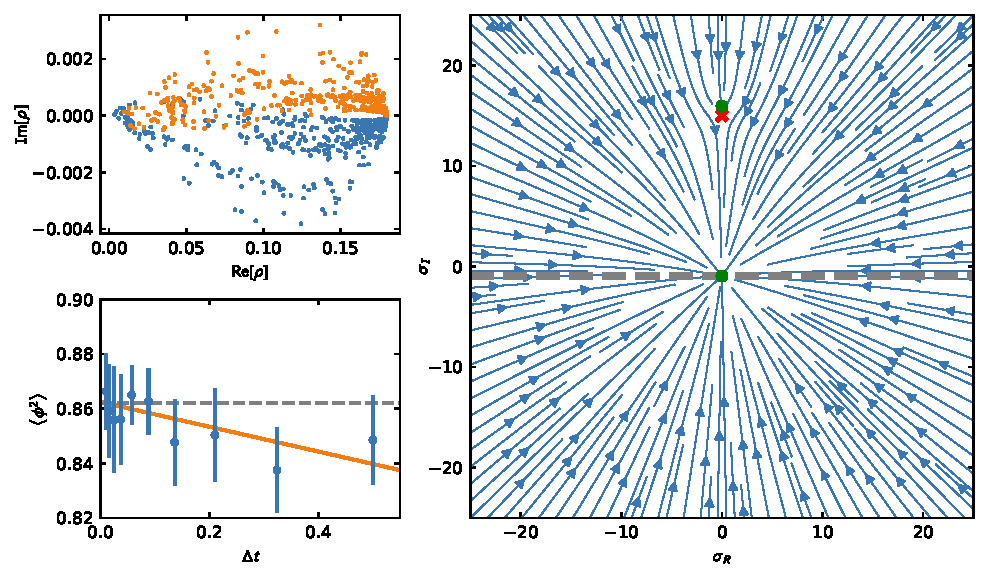
\includegraphics[width=\columnwidth]{./3mathunderpinnings/complex_plot.pdf}
   \caption{\label{fig:cl_stepsize}
   CL analysis for the action \equref{langevin_toy_continuum} with $\mu = 1.0$ and $\lambda = 0.4$, corresponding to the single well potential.
   (Upper left) Imaginary vs. real part of the complex weight in \equref{cl_bosonized_z}. Samples with ${\rm Re}[\sigma] > 0 $ and ${\rm Re}[\sigma] < 0$ are shown in orange and blue symbols respectively.
  (Lower left) Integration step dependence of the second moment $\langle \phi^2 \rangle$ as obtained with CL (symbols). The solid line represents a linear fit to the data in order to extrapolate to $\Delta t\to 0$ and the dashed line shows the exact result.
   (Right) Classical flow diagram with attractive fixed points (green dots) and the pole associated with the branch point of the action (red cross). The gray dashed line represents the domain of the equilibrium probability distribution.}
 \end{figure}

 It is instructive to investigate the sampled configurations by looking at the complex weight according to \equref{cl_bosonized_z}. This is shown in the upper left panel of \figref{cl_stepsize} where it becomes clear that the Langevin process now samples a complex quantity which is necessary to represent the correct answer. The coloring highlights the sampled configurations of $\sigma$ corresponding to regions with ${\rm Re}[\sigma] > 0 $ and ${\rm Re}[\sigma] < 0$.
 These two sets are connected through a point in configuration space which corresponds to a stationary point in the ``classical flow", i.e. the vanishing of the drift terms in \equref{cl_toy2_langevin}. {(The entire flow diagram is shown on the right panel of \figref{cl_stepsize}}). The attractive fixed point (marked by the lower green dot) pulls the field towards the connection point, while the noise induces fluctuations around that point, which occur mainly in the real component, as we have chosen to use only real noise in \equref{cl_toy2_langevin} (such that the only way the imaginary part can change is through the complex part of the drift). Thus, the imaginary component stays approximately constant during the Langevin evolution.

 The situation might change drastically if poles are encountered inside the domain of the distribution, which could lead to a breakdown of ergodicity, due in turn to a breakdown of holomorphicity of the action stated above (see also the discussion below). In the model considered here, we can find a pole at the point $\sigma = 6\tfrac{\mu}{\lambda}$, which corresponds to the branch-point of the action (marked by the red cross). At first glance this looks very dangerous as there is also an attractive stationary point (upper green dot) right next to the pole which would suggest faulty behavior. However, the imaginary part of the drift points away from the pole and even if a trajectory approaches this area of configuration space, fluctuations (in the real direction) will kick the process back into a stable trajectory that decays towards the attractive fixed point below. In equilibrium, the distribution will thus be confined to the gray dashed line far away from the pole, ensuring correct behavior (i.e. it is approximately shifted from the real axis by a constant offset). In fact, the existence of such an attractive fixed point is a necessary condition for the existence of an equilibrium distribution of the Langevin process \cite{CLZeroesFermionDet,Seiler2017StatusOfCL}. Luckily, this appears to be the case for systems of physical interest.



%%%%%%%%%%%%%%%%%%%%%%%%%%%%%%%%%%%
%%%%%%%%%%%%%%%%%%%%%%%%%%%%%%%%%%%
%%%%%%%%%%%%%%%%%%%%%%%%%%%%%%%%%%%
%%%%%%%%%%%%%%%%%%%%%%%%%%%%%%%%%%%
%%%%%%%%%%%%%%%%%%%%%%%%%%%%%%%%%%%

\subsection{Formal aspects and justification}

The CL process defines a random walk in a complexified manifold, such that for a given
configuration $\phi =  \phi_R + i\phi_I$ there is a well-defined probability $P[\phi_R,\phi_I,t]$ at time $t$.
For a given observable $\mathcal O$, there will be an expectation value
%
\beq
\langle \mathcal O \rangle_{P(t)}^{} \equiv
\int \mathcal D\phi_{R} \mathcal D\phi_I\ P[\phi_R,\phi_I,t] \CO[\phi_{R}+ i \phi_{I}].
\eeq
%
By virtue of the CL process, the real probability $P[\phi_R,\phi_I,t]$ obeys the FP equation:
%
\beq
\frac{\partial P}{\partial t} = L^{T} P \, ,
\eeq
%
where
%
\beq
L^T = \int {\rm d}\tau{\rm d}^dx\left\{ \frac{\delta}{\delta{\phi_R}}\left [N_R \frac{\delta}{\delta{\phi_R}} - K_R \right]
+ \frac{\delta}{\delta{\phi_I}}\left [N_I \frac{\delta}{\delta{\phi_I}} - K_I \right]\right\}\,.
\eeq
%
It is not obvious {\it a priori} whether this process would reproduce the desired expectation values of the physical observables,
i.e. whether $\langle \mathcal O \rangle_{P(t)}^{}$ actually corresponds to the physical expectation value of the theory,
at least in the large-$t$ limit. In fact, it is not even clear that the process would converge and if it does, whether it converges to the
correct answer. Indeed, following the steps outlined above for the case of real Langevin, one finds that the resulting FP Hamiltonian
is neither self-adjoint nor positive semidefinite, such that the proof of convergence to the desired probability distribution is spoiled.

The fundamental question underlying the validity of the CL approach is the relation between the CL distribution $P[\phi_R,\phi_I,t]$
and the desired complex distribution $\rho[\phi]$ in \equref{complex_p}. The latter defines the physics of interest and is a fixed point of its own FP equation
%
\beq
\label{Eq:LTrho}
\frac{\partial \rho}{\partial t} = L^{T}_0 \rho\, ,
\eeq
%
where
%
\beq
L^T_0 = \int {\rm d}\tau{\rm d}^dx\ \frac{\delta}{\delta{\phi_R}}\left [ \frac{\delta}{\delta{\phi_R}} +  \frac{\delta S}{\delta{\phi_R}}\right],
\eeq
%
which is obtained by temporal differentiation of
%
\beq
\langle \mathcal O \rangle_{\rho(t)}^{}  \equiv \int \mathcal D\phi_{R}\ \rho[\phi_R,t] \CO[\phi_{R}].
\eeq
%
Again, the absence of boundary terms at infinity when integrating by parts was assumed. More specifically, the crucial question is whether
%
\beq
\label{Eq:realcomplexprobabilities}
\langle \mathcal O \rangle_{P(t)}^{}  = \langle \mathcal O \rangle_{\rho(t)}^{}\, ,
\eeq
%
holds.

In Refs.~\cite{AartsPRD81054508, 2011EurPhysJC711756} it was shown how the desired relationship \equref{realcomplexprobabilities} can be proven for holomorphic observables, as long as the action and the associated drift are holomorphic functions of $\phi$. The proof relies on analyzing the behavior of
%
\beq
  F(t,\tau) = \int \mathcal D \phi_{R} \mathcal D\phi_{I}\ P[\phi_{R}, \phi_{I},t-\tau]\CO [\phi_{R} + i\phi_{I},\tau],
\eeq
%
where $0 \leq \tau \leq t$. The function $F(t, \tau)$ interpolates between the two expectation values of interest:
%
\bea
F(t,0) = \langle \mathcal O \rangle_{P(t)}^{}, &  &  F(t,t) = \langle \mathcal O\rangle_{\rho(t)}^{}.
\eea
%
where we have assumed that the initial conditions are chosen as
%
\beq
\label{Eq:InitialConditions}
P (\phi_{R}, \phi_{I}, 0) = \rho[\phi_{R}, 0]\delta(\phi_{I} - \phi_{I,0}).
\eeq
%
We find that
%
\beq
F(t,0) = \int \mathcal D \phi_{R} \mathcal D\phi_{I} P[\phi_{R}, \phi_{I}, t]\CO [\phi_{R} + i\phi_{I},0] = \langle \mathcal O \rangle_{P(t)}^{},
\eeq
%
while, using the initial conditions of \equref{InitialConditions},
%
\beq
F(t,t) = \int \mathcal D \phi_{R} \mathcal D\phi_{I} P[\phi_{R}, \phi_{I},0] \CO [\phi_{R} + i\phi_{I},t] =
\int \mathcal D \phi_{R}\ \rho[\phi_{R}, 0] \CO [\phi_{R} + i\phi_{I,0},t] =  \langle \mathcal O \rangle_{\rho(t)}^{},
\eeq
%
where we have used \equref{LTrho} to shift the Langevin evolution operator from $\mathcal O$ to $\rho$ by transposition
(which involves integration by parts).

If $F(t,\tau)$ is independent of $\tau$, then \equref{realcomplexprobabilities} holds, and
the Langevin method is formally shown to be valid for complex-valued variables, i.e. to converge
to the correct physical answers (assuming it converges). Naturally, this statement assumes that the expectation
values in \equref{realcomplexprobabilities} agree at $t=0$, which can be ensured by choosing the initial condition
of the Langevin process as above. The $\tau$ derivative of $F(t,\tau)$ involves an integration by parts:
%
\beq
\label{Eq:CL_IBP}
  \frac{\partial}{\partial \tau} F(t,\tau) =
  \int \mathcal D \phi_{R} \mathcal D\phi_{I}\left\{ P[\phi_{R}, \phi_{I},t-\tau]  L \CO [\phi_{R} + i\phi_{I},\tau]- L^{T}
  P[\phi_{R}, \phi_{I},t-\tau]\CO [\phi_{R} + i\phi_{I},\tau]\right\} ,
\eeq
%
where $L$ is the Langevin operator and $L^{T}$ its adjoint. If integration by parts is carried out and -- importantly --
the boundary terms are zero, then $\frac{\partial}{\partial \tau} F(t,\tau) = 0$. If the decay of
%
\beq
P[\phi_{R}, \phi_{I},t-\tau] \CO [\phi_{R} + i\phi_{I},\tau] \, ,
\eeq
%
and its derivatives is not fast enough to ensure that the boundary terms will vanish, then it cannot be guaranteed that
the expectation values of the quantities of interest obtained via a Langevin process will converge to the correct
values~\cite{AartsPRD81054508, 2011EurPhysJC711756}.

While the condition of fast decay was recognized in~\cite{AartsPRD81054508, 2011EurPhysJC711756},
the precise rate was not immediately clear. In Ref.~\cite{CLJustificationPRD94114515}, the above arguments were
reviewed by considering a finite step-size in Langevin time. It was then found that the above integration by parts is
valid if the probability distribution of the drift term falls off faster than any power at large drift magnitude.
In practice, it is very difficult to establish the behavior of \equref{CL_IBP}, but it is perfectly possible to study
the probability distribution of the drift and establish whether the decay is exponential.


%%%%%%%%%%%%%%%%%%%

\subsection{\label{sect:CLchallenges}Challenges}

The challenges faced by the CL method can be roughly divided into two kinds: mathematical and practical, which
naturally have some overlap. In this subsection we attempt to summarize the current understanding of these issues.

\subsubsection{Mathematical aspects: convergence, correctness, boundary terms, and ergodicity}

\begin{itemize}
\item {\it Convergence --} Without a doubt, the biggest challenge for CL is the lack of general mathematical proofs, the previous section notwithstanding.
More specifically, as pointed out most recently in Ref.~\cite{Seiler2017StatusOfCL}, it remains unknown whether the Langevin operators defined
above as $L$, $L_0$, $L^T$, $L_0^T$ properly define unique stochastic processes, although in practice this is not typically an issue.
Crucially, it remains unknown under what conditions the positive measure
$P[\phi_{R}, \phi_{I},t]$ converges to an equilibrium measure, although (again) there is substantial numerical evidence that such an equilibrium
measure exists in many cases of interest.

\item {\it Correctness --} The above issues aside, CL has been shown to fail in certain cases (due either to failure to converge or convergence to the wrong answer),
but also appears to work in scenarios that lie outside the holomorphic-action regime mentioned above.
In cases of failure, the behavior has been traced back to insufficient {\it decay at infinity},
or to a breakdown of ergodicity due to {\it poles in the action} (which should be expected in fermionic
systems as the fermion determinant will vanish at specific points, thus leading to meromorphic drifts).

\begin{itemize}
\item {\it Boundaries at infinity --} The behavior of boundaries at infinity is a relevant question for models in relativistic and non-relativistic physics.
In particular, for gauge theories the complexification of the link variables leads to non-compact groups, e.g. SU(3) becomes SL(3,C).
As we explain in \secref{NRQFT}, a similar effect is seen in nonrelativistic physics when using compact HS transformations.
In either case, merely assuming that the derivative of $F(t,\tau)$ in \equref{CL_IBP} vanishes is a bad idea. For that to happen,
the solutions to the FP equation must fall off sufficiently quickly along non-compact directions in the (complexified) space of field
configurations (see in particular Refs.~\cite{PRDSalcedoCL2016, PhysRevD.99.014512} for a recent and insightful discussion of an
exactly solvable case). That property is very difficult to determine {\it a priori}, but can be checked {\it a posteriori} following the arguments of
Ref.~\cite{CLJustificationPRD94114515}. Case studies show
that in many cases, while the solutions fall off faster than exponentially in the real directions, the decay in the imaginary directions may be
insufficient~\cite{AartsPRD81054508}. Such an insufficient decay at infinity can also lead to the so-called excursion problem, which we
discuss below.

\item {\it Poles and ergodicity --} For fermionic actions where poles appear naturally, the results for the holomorphic case can be used, provided that
a region around the poles is cut out~\cite{CLZeroesFermionDet}. That procedure is justified as long as the probability measure vanishes around
those poles sufficiently fast; in other words, one has to address the boundaries around the poles alongside those at infinity mentioned above.
A detailed study of incorrect convergence due to poles in the drift function showed that the location of these poles,
the decay of the drift function, and the behavior of the observables in the region near the poles all played a role in whether the method
would return correct results~\cite{CLZeroesFermionDet, CLJustificationPRD94114515}.

As mentioned above, a re-examination of the conditions for correctness in Refs.~\cite{PhysRevD.92.011501, CLJustificationPRD94114515}
revealed that failure of CL that in some cases has been attributed to the excursion and singular drift problems are actually due to the drift function
falling off too slowly.

It was argued in Ref.~\cite{Hayata:2015lzj}, using a semiclassical analysis, that when more than one saddle point in the complex plane contributes to the
ensemble averages, the CL method can lead to incorrect answers due to the different complex phases associated with each saddle point.
The interference of these complex phases is an essential in phenomena such as the Silver Blaze phenomenon and real-time dynamics.

\end{itemize}

\end{itemize}


%%%%%%%%%%%%%%%%%%%%%
\subsubsection{Practical aspects: numerical instabilities, gauge cooling, dynamic stabilization, and regulators}

On the practical side, several strategies have been identified to tackle specific issues.

\begin{itemize}

\item {\it Instabilities --} One of the issues recognized early on (in fact, since the 1980s; see e.g.~\cite{Ambjorn:1985cv, Ambjorn:1985iw}) is the appearance of instabilities in the form of runaway trajectories
along the CL evolution. These can become very frequent so as to completely spoil a calculation performed
at fixed step size. In Ref.~\cite{AARTS2010154}, the need for adaptive step size integration of the complex Langevin equations
was identified. It was found that such an approach provides a full solution to the problem of instabilities and has thus
become the standard for CL calculations.

\item {\it Boundaries at infinity --} A separate but crucial issue for correctness, mentioned above, is that of insufficient decay at infinity. In practice, it can lead to uncontrolled
excursions of the CL process into the complex plane, making calculations unstable. To that end, a few practical solutions have been explored which
have, in some cases been mathematically well justified.

\begin{itemize}
\item {\it Gauge cooling}~\cite{SeilerGaugeCooling, Bongiovanni:2013nxa, PhysRevD.92.085020, Nagata:2015uga, Nagata:2016alq}
is one example of such practical solutions which, though necessary, is often not sufficient. It remains, however, the best
understood approach from a mathematical perspective~\cite{Nagata:2015uga}: In contrast to the next two items, gauge cooling is a
mathematically exact procedure. The idea is that at each Langevin step, one can make a gauge transformation (in the extended
non-compact group, say SL(3,C)) to keep the link variables close to the compact subgroup SU(3).


\item {\it Dynamic stabilization}~\cite{Aarts:2016qhx, Lattice2016AttanasioJager, Lattice2017AttanasioJager, Attanasio2019} was developed to further aid with
the excursion problem. The essential idea of this approach is to add a term to the Langevin drift $K$ in the schematic form
%
\beq
K \to -D S + i \alpha_{DS} M,
\eeq
%
where $-D S$ is the standard CL drift, $\alpha_{DS}$ is a control parameter, and $M$ acts only in the non-SU(3) directions and grows rapidly
with the distance from the SU(3) manifold. The above modification to the Langevin evolution cannot be derived from
the action but it vanishes in the continuum limit and prevents large excursions into the complex plane.

\item {\it Regulators} or modified actions, first appeared in a nonrelativistic application, namely
Ref.~\cite{PRD95094502}. They were also discussed more recently in Ref.~\cite{PhysRevD.99.014512} and the idea is similar to dynamic
stabilization, except that the resulting modifications on the Langevin equations are directly derived from the action. In both of those works, the
modification consisted of adding a term of the form $\xi \phi^2$, with the prescription that one should examine the behavior
of the CL results in the limit $\xi \to 0$. While the advantages of such a practical solution were clear, it is by no means a full solution and
in many cases -- especially at strong coupling or low temperatures -- it is not possible to make $\xi$ small and obtain a converging calculation.

\end{itemize}

%Another concerning and not yet well-understood problem that can occur occasionally in the application of CL is the convergence
%of the algorithm to a stationary distribution which is not the correct solution~\cite{GaustererNPA1998, AartsPRD81054508}. The
%probability distribution density of the process must converge for CL to work, but even if it converges, one must determine
%whether it correctly simulates the desired system.

\item Quantum field theories can be cast in terms of differential equations rather than path integrals; this is called the Schwinger action
principle. A specific set of differential equations resulting from this principle is the Schwinger-Dyson equations, and these involve
variations with respect to the source fields. Of the many solutions to this set of differential equations, only one at most corresponds
to the Feynman path integral.  It appears that the CL method is able to converge to multiple stationary distributions, and while at
most one of those distributions corresponds to the desired distribution, it has been shown that these stationary distributions of the
complex Langevin equation satisfy the Schwinger-Dyson equations~\cite{PhysRevD75045007, xue1986}.

The initial conditions appear to play a role in this behavior: CL converges to certain solutions of the Schwinger-Dyson equation with
one set of initial conditions and to another with a different set, and for certain conditions CL does not converge at all
~\cite{GuralnikNPB200905503213, Salcedo1993SpuriousCLSolutions}. The role of the Schwinger-Dyson equations in the presence of
zeros of the complex density $\rho$ was analyzed in detail in Ref.~\cite{Salcedo:2018fvt}. Further study of the convergence of CL to incorrect solutions
must be an integral part of the understanding and application of this method to systems with complex actions.



\end{itemize}

\end{document}
